\documentclass[12pt,]{article}
\usepackage[utf8]{inputenc}
\usepackage[T1]{fontenc}
\usepackage{mathptmx}
\usepackage{geometry}
\usepackage{mathtools}
\usepackage[english]{babel}
\usepackage{graphicx}
\usepackage{subcaption}
\usepackage{stackengine}
\usepackage[os=win]{menukeys}
\usepackage{hyperref}
\usepackage{minted}
\usepackage{xcolor}
\usepackage{tikz}
\usepackage[yyyymmdd,hhmmss]{datetime}
\usepackage{etoolbox}
\usepackage[inline]{enumitem}
\usepackage{pdfpages}

\newcommand{\WindowsLogo}{\raisebox{-0.1em}{
\includegraphics[height=0.8em]{images/logo/Windows_3_logo_simplified}}}
%\newcommand{\PowerLogo}{\raisebox{-0.1em}{\includegraphics[height=0.8em]{images/logo/power}}}
\newcommand{\WinKey}{\keys{\WindowsLogo}}
\newcommand{\PowerKey}{\keys{\PowerLogo}}

\patchcmd{\thebibliography}{\section*{\refname}}{}{}{}

\newcommand{\ShowOsVersion}{
	\immediate\write18{\unexpanded{foo=`uname -sro` && echo "${foo}" > tmp.tex}}
	\input{tmp}\immediate\write18{rm tmp.tex}
}

\newcommand{\ShowTexVersion}{
	\immediate\write18{\unexpanded{foo=`pdflatex -version | head -n1 | cut -d' ' -f1,2` && echo "${foo}" > tmp.tex}}
	\input{tmp}\immediate\write18{rm tmp.tex}
}

\addto\captionsenglish{\renewcommand{\contentsname}{Daftar Isi}}
\addto\captionsenglish{\renewcommand{\figurename}{Gambar}}

\hypersetup{
	colorlinks=true, %set true if you want colored links
	linktoc=all,     %set to all if you want both sections and subsections linked
	linkcolor=blue,  %choose some color if you want links to stand out
	urlcolor=blue,   %url color
}

\geometry{
	a4paper,
	left=10mm,
	right=10mm,
	top=10mm,
	bottom=15mm,
}

\title{\LARGE \bf
	Laporan Pengujian Unit Speech/Whisper Test\\
	(dengan perangkat DAQ National Instrument)
}

\author{Achmadi ST MT}

\date{}

\hypersetup{citecolor=black}

\definecolor{LightGray}{gray}{0.95}

%\pagecolor[rgb]{0.1,0.1,0.1}
%\color[rgb]{1,1,1}

\begin{document}
	\thispagestyle{empty}
	\pagestyle{empty}

	\begin{titlepage}
		\centering
		\vfill
		\vfill
		\maketitle
		\vfill
		
\includegraphics[width=200pt]{images/logo/logoviblab}
		\vfill
		\vfill
		Update: {\today} \currenttime \\
	\end{titlepage}

	%%%%%%%%%%%%%%%%%%%%%%%%%%%%%%%%%%%%%%%%%%%%%%%%%%%%%%%%%%%%%%%%%

	\newpage
	\tableofcontents

	%%%%%%%%%%%%%%%%%%%%%%%%%%%%%%%%%%%%%%%%%%%%%%%%%%%%%%%%%%%%%%%%%

	\newpage
	\section{Pendahuluan}

	subsection{Tujuan}

	Tujuan kegiatan pengukuran ini meliputi:
	\begin{itemize}
		\item Mengetahui nilai dB SPL untuk Elitech Speech Test menggunakan Headphone
		\item Mengetahui nilai dB SPL untuk Elitech Wishper Test menggunakan Headphone
		\item Mengetahui nilai dB SPL untuk Elitech Speech Test menggunakan Speaker
		\item Mengetahui nilai dB SPL untuk Elitech Wishper Test menggunakan Speaker
	\end{itemize}

	\subsection{Waktu dan Tempat}

	Seluruh kegiatan dilakukan di Ruang Semi-Unechoic Laboratorium Vibrasi dan Akustik
	Departemen Teknik Fisika Institut Teknologi Sepuluh Nopember Surabaya.
	Kegiatan pengukuran dilakukan pada bulan Oktober 2021.

	%%%%%%%%%%%%%%%%%%%%%%%%%%%%%%%%%%%%%%%%%%%%%%%%%%%%%%%%%%%%%%%%%

	\newpage
	\section{Persiapan}

	Kegiatan persiapan disini meliputi:
	\begin{itemize}
		\item Modifikasi file Audio.
		\item Kalibrasi instrumen ukur.
		\item Pengukuran audio latar ruangan.
	\end{itemize}

	Instrumen yang digunakan meliputi:
	\begin{itemize}
		\item miniDSP EARS, berupa replika telinga karet dengan mikrofon, box DSP, dan antarmuka USB.
		Website produk:\\
		\url{https://www.minidsp.com/products/acoustic-measurement/ears-headphone-jig}

		\begin{figure}[!ht]
			\centering
			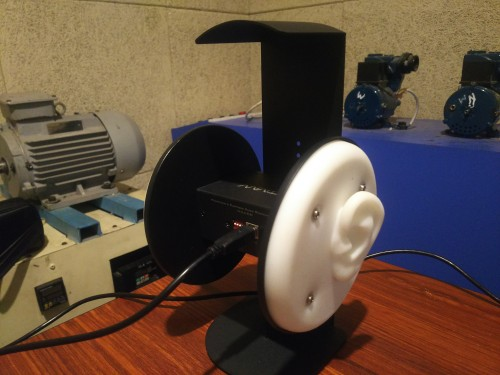
\includegraphics[width=200pt]{images/ears}
			\caption{miniDSP EARS}
		\end{figure}

		Disini instrumen EARS hanya digunakan sebagai model telinga saja,
		namun output data USB tidak digunakan.

		\item National Instrument Microphone Array

		Instrumen ukur ini berupa Microphone Array yang terhubung dengan Unit DAQ buatan National Instrumen.
		Kemudian Unit DAQ terhubung ke laptop via USB.
		Representasi Data ditampilkan dengan software LabView.
		Selanjutnya paket instrumen ini disebut NI saja.

		\begin{figure}[!ht]
			\centering
			\begin{subfigure}[b]{0.3\textwidth}
				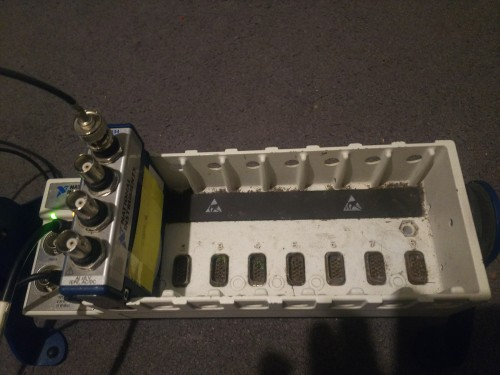
\includegraphics[width=\textwidth]{images/ni_daq}
				\caption{Unit DAQ}
			\end{subfigure}
			\begin{subfigure}[b]{0.3\textwidth}
				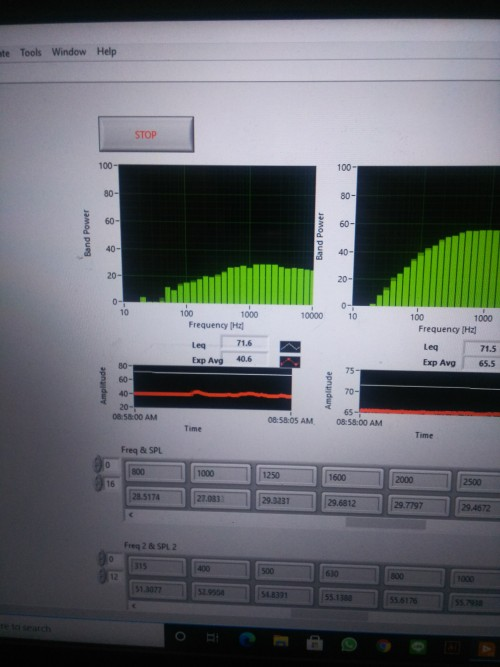
\includegraphics[width=\textwidth]{images/labview_0}
				\caption{LabView}
			\end{subfigure}
			\caption{NI DAQ}
		\end{figure}
	
		\item SLM Onnosokki sebagai pembanding dalam pengukuran latar.
		SLM telah terkalibrasi dan telah dicek dengan kalibrator.
		Untuk selanjutnya paket instrumen ini disebut SLM saja.

		\begin{figure}[!ht]
			\centering
			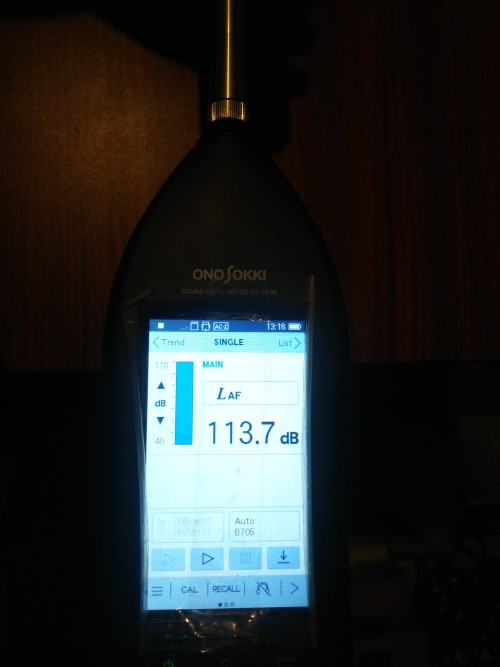
\includegraphics[width=150pt]{images/slm_calib}
			\caption{SLM Onnosokki}
		\end{figure}
		
	\end{itemize}

	\subsection{File Audio}
	
	Dalam SDCard yang terinstal di unit prototype, tersedia 20 file audio MP3 dengan pembagian:
	\begin{itemize}
		\item File nomor 01 hingga 10 untuk Speech Test.
		\item File nomor 11 hingga 20 untuk Wishper Test.
	\end{itemize}
	
	Dipilih file 01 dan 11.
	Kemudian kedua file tersebut dibuang \textit{silence} di antara 5 kata pertama.
	Selanjutnya sisa \textit{track} dibuang.
	Tujuannya adalah untuk bisa diputar \textit{looping} dengan meminimumkan \textit{silence}.

	\begin{figure}[!ht]
		\centering
		\begin{subfigure}[b]{0.49\textwidth}
			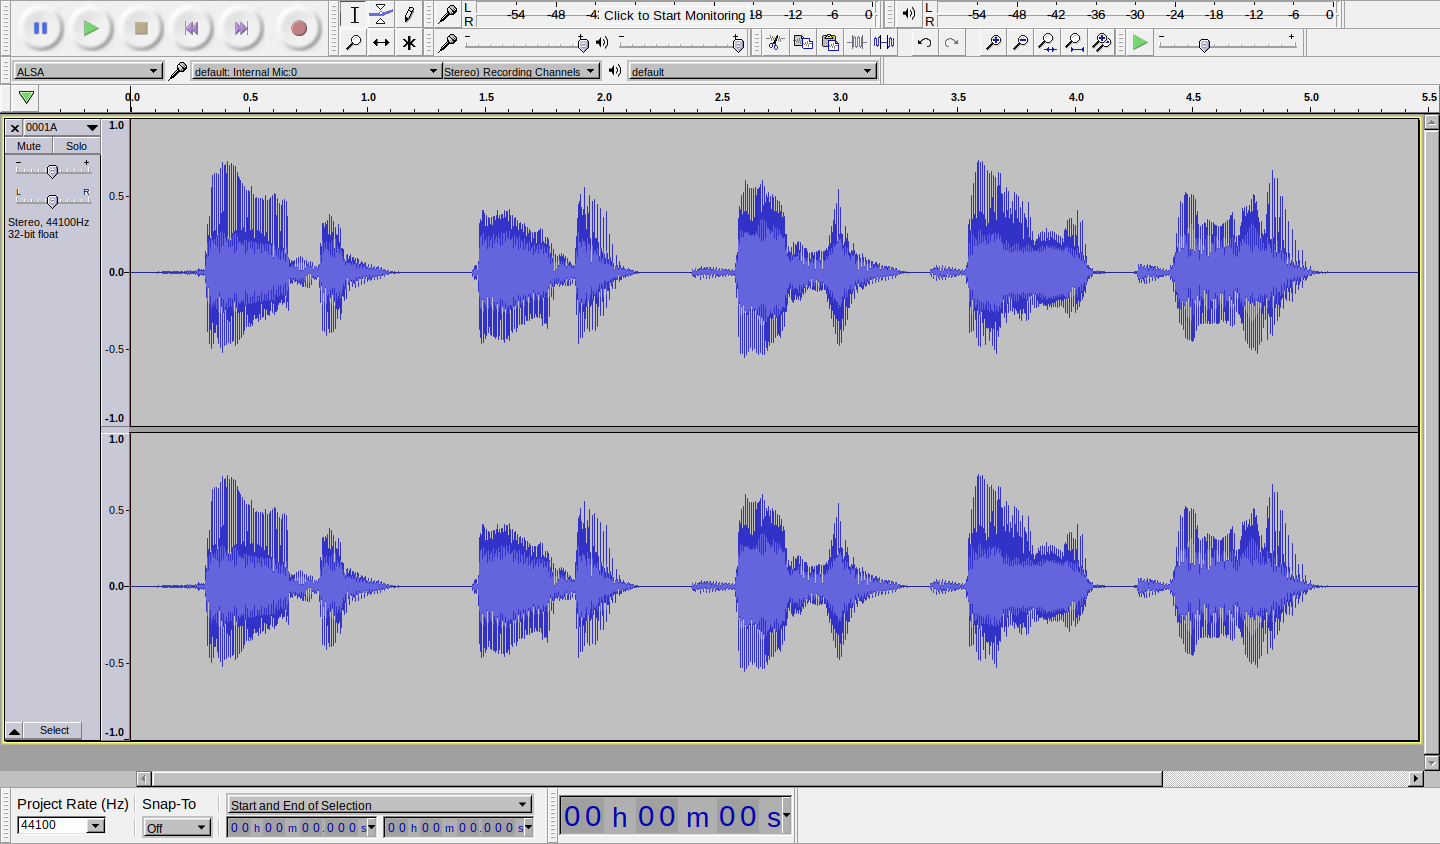
\includegraphics[width=\textwidth]{images/elitech_testAudioSpeech}
			\caption{Speech}
		\end{subfigure}
		\begin{subfigure}[b]{0.49\textwidth}
			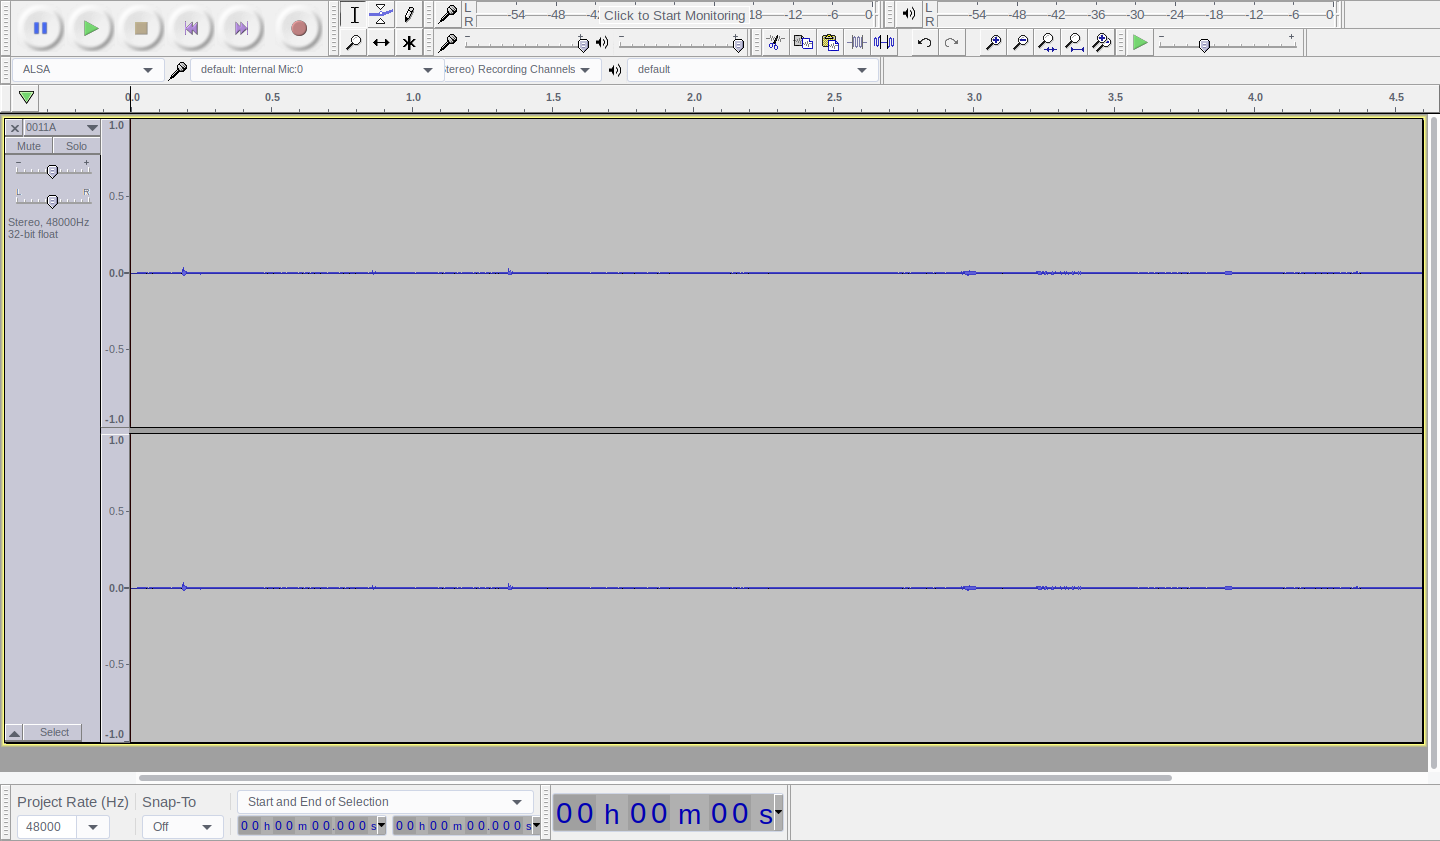
\includegraphics[width=\textwidth]{images/elitech_testAudioWhisperOri}
			\caption{Whisper}
		\end{subfigure}
		\caption{Audio Track}
	\end{figure}

	\newpage
	Perlu diketahui bahwa Audio Whisper memiliki level bit sangat rendah mendekati silence.
	
	\begin{figure}[!ht]
		\centering
		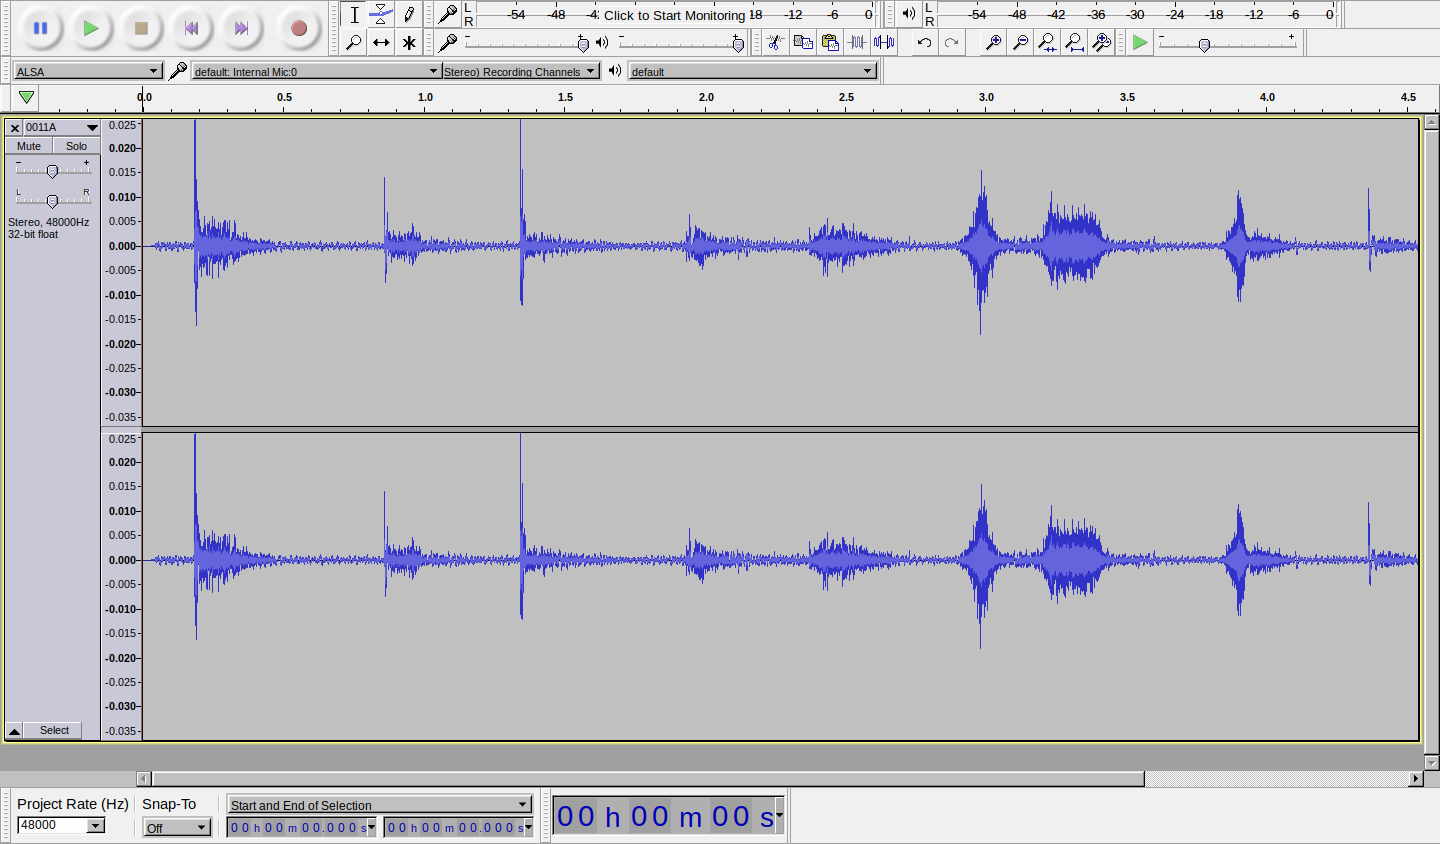
\includegraphics[width=250pt]{images/elitech_testAudioWhisper}
		\caption{Track Audio untuk Whisper (Zoomed)}
	\end{figure}
	
	Kemudian melihat analisa frekuensi:
	
	\begin{figure}[!ht]
		\centering
		\begin{subfigure}[b]{0.25\textwidth}
			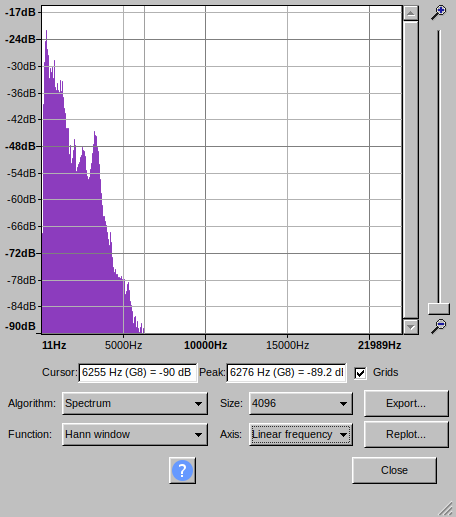
\includegraphics[width=\textwidth]{images/elitech_testAudioSpeechFreq}
			\caption{Speech}
		\end{subfigure}
		\begin{subfigure}[b]{0.25\textwidth}
			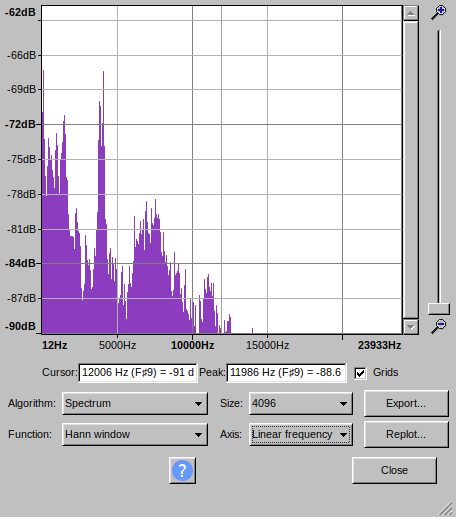
\includegraphics[width=\textwidth]{images/elitech_testAudioWhisperFreq}
			\caption{Whisper}
		\end{subfigure}
		\caption{Analisa Frekuensi}
	\end{figure}

	\subsection{Pengukuran latar}
	
	Pengukuran latar dilakukan dengan Mic dan SLM Onosokki.
	
	\begin{figure}[!ht]
		\centering
		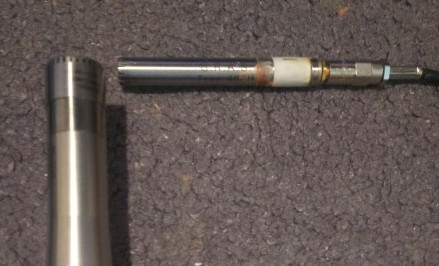
\includegraphics[width=300pt]{images/ni_noise}
		\caption{Pengukuran Latar}
	\end{figure}

	\newpage
	Masing-masing menunujukkan nilai kisaran 40dB SPL.
	
	\begin{figure}[!ht]
		\centering
		\begin{subfigure}[b]{0.25\textwidth}
			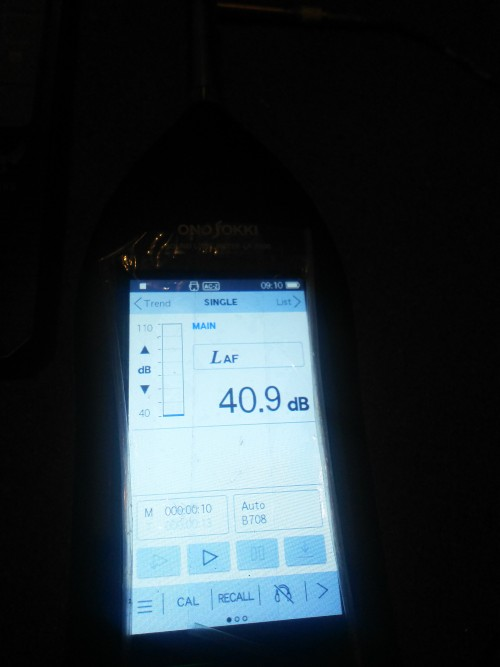
\includegraphics[width=\textwidth]{images/noise_slm}
			\caption{SLM}
		\end{subfigure}
		\begin{subfigure}[b]{0.25\textwidth}
			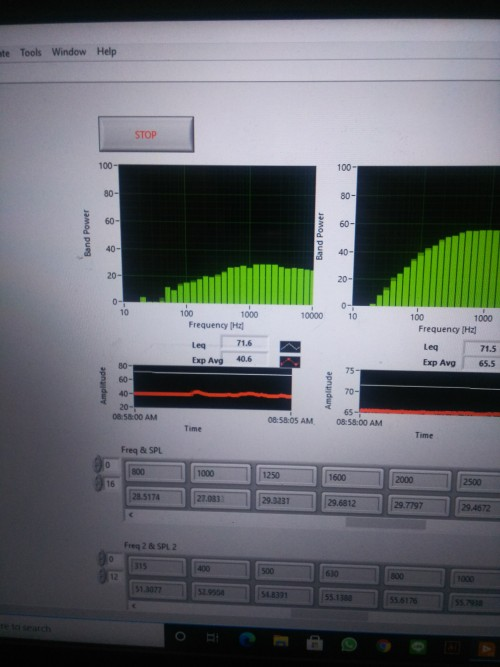
\includegraphics[width=\textwidth]{images/noise_ni}
			\caption{NI}
		\end{subfigure}
		\caption{Pengukuran Latar}
	\end{figure}

	%%%%%%%%%%%%%%%%%%%%%%%%%%%%%%%%%%%%%%%%%%%%%%%%%%%%%%%%%%%%%%%%%
	
	\newpage
	\section{Hasil Pengukuran}
	
	Hasil Pengukuran dibagi dalam dua kategori,menggunakan Headphone dan Speaker.
	
	\subsection{Headphone}
	
	Untuk pengukuran menggunakan headphone, microphone yang digunakan diselipkan ke dalam telinga EARS.
	
	\begin{figure}[!ht]
		\centering
		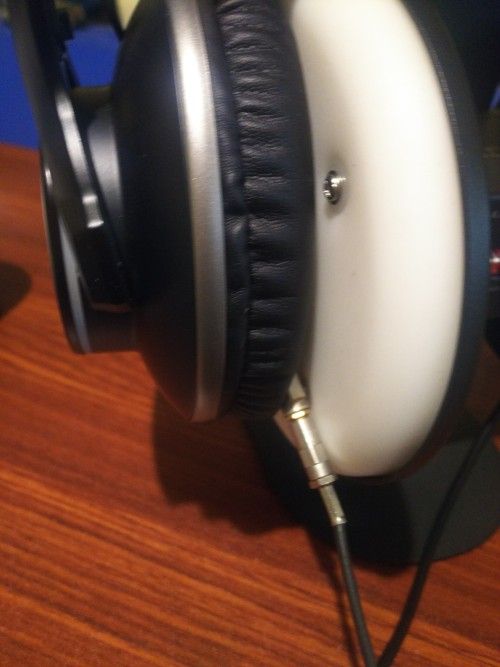
\includegraphics[width=150pt]{images/ukur_mic}
		\caption{Penempatan Microphone}
	\end{figure}

	Nilai dB SPL dasar di dalam telinga EARS (tertutup oleh headphone) berada di kisaran 36 dB SPL.
	
	\begin{figure}[!ht]
		\centering
		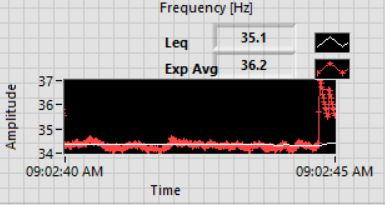
\includegraphics[width=200pt]{images/eli0}
		\caption{Loudness sebelum ada output.}
	\end{figure}
	
	Kemudian setup prototype:
	
	Berikut langkah-langkah persiapan yang dijalankan:
	\begin{enumerate}
		\item Siapkan prototype di atas meja.
		
		\begin{figure}[!ht]
			\centering
			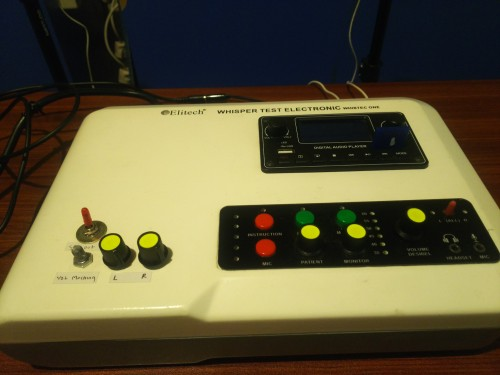
\includegraphics[width=200pt]{images/prototype}
			\caption{Prototype Test}
		\end{figure}
		
		\newpage
		\item Sambungkan koneksi output yang dubutuhkan.
		
		\begin{figure}[!ht]
			\centering
			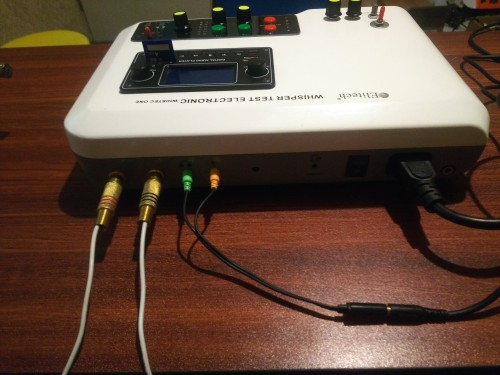
\includegraphics[width=200pt]{images/kabel_out}
			\caption{Koneksi Output}
		\end{figure}
		
		\item Nyalakan unit dan pastikan file MP3 yang di \textit{loop-play} sudah sesuai
		
		\begin{figure}[!ht]
			\centering
			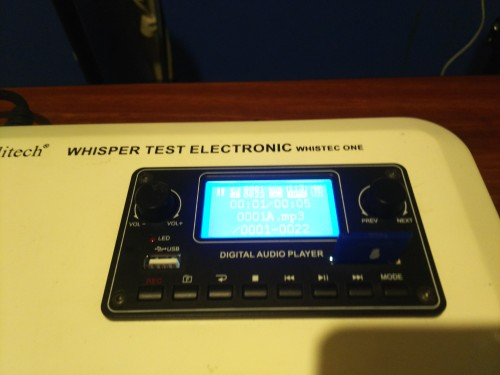
\includegraphics[width=175pt]{images/loopplay}
			\caption{File Loop-Play}
		\end{figure}
	
		\item Maksimalkan semua volume. Pengujian akan dilakukan dengan knob pengaturan kuantisasi loudness.
		
		\begin{figure}[!ht]
			\centering
			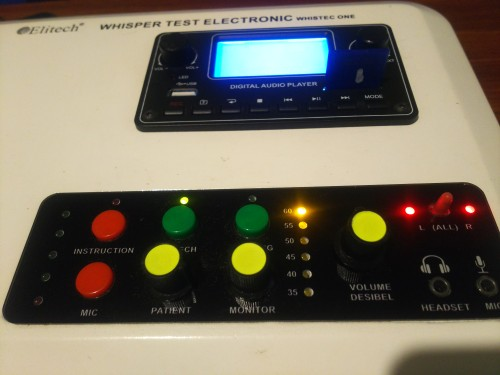
\includegraphics[width=150pt]{images/loudset}
			\caption{Pengaturan Kuantisasi Loudness}
		\end{figure}
		
		\item Sambungkan Headphone ke Prototype.
		Nilai dapat dibaca pada tampilan LabView:
		
		\begin{figure}[!ht]
			\centering
			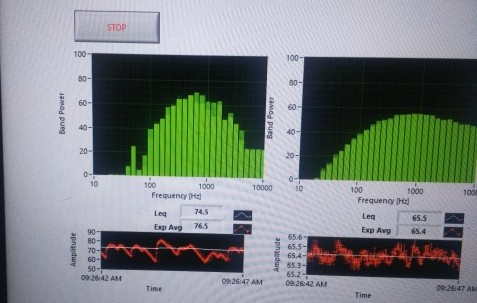
\includegraphics[width=200pt]{images/ni_ukur}
			\caption{Tampilan Pengukuran}
		\end{figure}
		
	\end{enumerate}

	\newpage
	Berikut hasil ukur untuk prototype A dan prototype B (dengan output speaker)
	
	\begin{itemize}
		\item Prototype-A
		
		Disajikan dalam bentuk tabel (dalam dB SPL):
		\begin{center}
			\begin{tabular}{|c|c|c|c|c|c|c|}
				\hline
				Output & 60 & 55 & 50 & 45 & 40 & 35\\ [0.5ex]
				\hline\hline
				Speech & 77.2 & 68.2 & 58.4 & 48.6 & 46.6 & 40.2 \\
				\hline
				Whisper & 39.8 & 36.2 & 36.3 & 36.1 & 36.2 & 36.1 \\
				\hline
			\end{tabular}
		\end{center}

		\item Prototype-B (yang dilengkapi output Speaker)
		
		Disajikan dalam bentuk tabel (dalam dB SPL):
		\begin{center}
			\begin{tabular}{|c|c|c|c|c|c|c|}
				\hline
				Output & 60 & 55 & 50 & 45 & 40 & 35\\ [0.5ex]
				\hline\hline
				Speech & 75.4 & 65.6 & 54.4 & 51.6 & 50.6 & 43.2 \\
				\hline
				Whisper & 42.8 & 36.4 & 36.1 & 36.2 & 36.1 & 36.1 \\
				\hline
			\end{tabular}
		\end{center}
	\end{itemize}

	Untuk pengukuran Prototype-B dengan speaker, setup mic NI dan speaker:
	
	\begin{figure}[!ht]
		\centering
		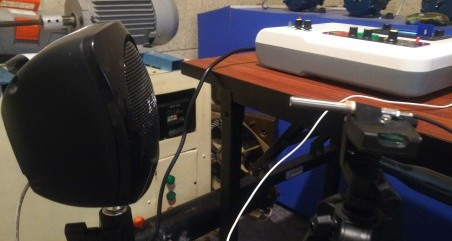
\includegraphics[width=200pt]{images/ukur_speaker}
		\caption{Penempatan Mic terhadap Speaker}
	\end{figure}

	Kemudian dengan metode setup prototype yang sama seperti sebelumnya,
	disajikan dalam bentuk tabel (dalam dB SPL):
	\begin{center}
		\begin{tabular}{|c|c|c|c|c|c|c|}
			\hline
			Output & 60 & 55 & 50 & 45 & 40 & 35\\ [0.5ex]
			\hline\hline
			Speech & 92.4 & 86.6 & 74.6 & 67.8 & 64.5 & 56.8 \\
			\hline
			Whisper & 55.6 & 48.6 & 37.9 & 36.6 & 36.5 & 36.1 \\
			\hline
		\end{tabular}
	\end{center}

	\color{red} \textbf{CATATAN:}
	Selain nilai output audio whisper yang terlalu kecil,
	juga headphone/speaker mengeluarkan derau pada frekuensi kisaran 1kHz.
	Loudness derau ini terdengar lebih tinggi ketimbang audio whisper itu sendiri.
	Sehingga pengukuran dibawah skala 55 akan rancu karena tenggelam terhadap derau audio itu sendiri.

\end{document}
